\documentclass[10pt,twoside]{article}
\usepackage[ngerman]{babel}
\usepackage[utf8]{inputenc}
\usepackage{textcomp,gensymb}
\usepackage{longtable}
\usepackage{lscape}
%\usepackage[latin1]{inputenc}
\usepackage{amsmath,thmtools}
\usepackage{siunitx}
\usepackage{enumitem} 
\usepackage{array}
\usepackage{amstext}
\usepackage{amssymb}
\usepackage{stmaryrd}
\usepackage{verbatim}
\usepackage{mathrsfs}
\usepackage{extarrows}
\usepackage[arrow, matrix, curve]{xy}
\usepackage[centering,includeheadfoot,top=25mm, left=40mm, right=25mm, bottom=30mm]{geometry}
\usepackage{gensymb}
\usepackage{graphicx}
\usepackage{framed}
\usepackage[usenames,dvipsnames]{xcolor}
\usepackage{float}
\usepackage{sidecap}
\usepackage{tikz,lipsum,lmodern}
\usepackage{wrapfig} % Allows wrapping text around tables and figures
\usepackage{import}
\usepackage{fancyhdr}
\usepackage{fancybox}
\usepackage{caption}
\usepackage{subcaption}
\usepackage{esint}
\parskip 10pt
\parindent 0pt
\DeclareGraphicsRule{.tif}{png}{.png}{`convert #1 `basename #1 .tif`.png} 
\makeindex
\usepackage[colorlinks,pdfpagelabels,pdfstartview = FitH,bookmarksopen = true,bookmarksnumbered = true,linkcolor = black,plainpages =false,hypertexnames = false,citecolor = black] {hyperref}
\makeatletter
\def\@tocline#1#2#3#4#5#6#7{\relax
  \ifnum #1>\c@tocdepth % then omit
  \else
    \par \addpenalty\@secpenalty\addvspace{#2}%
    \begingroup \hyphenpenalty\@M
    \@ifempty{#4}{%
      \@tempdima\csname r@tocindent\number#1\endcsname\relax
    }{%
      \@tempdima#4\relax
    }%
    \parindent\z@ \leftskip#3\relax \advance\leftskip\@tempdima\relax
    \rightskip\@pnumwidth plus4em \parfillskip-\@pnumwidth
    #5\leavevmode\hskip-\@tempdima
      \ifcase #1
       \or\or \hskip 1em \or \hskip 2em \else \hskip 3em \fi%
      #6\nobreak\relax
    \dotfill\hbox to\@pnumwidth{\@tocpagenum{#7}}\par
    \nobreak
    \endgroup
  \fi}
  \setcounter{tocdepth}{3}
\makeatother
%%%%%%%%%%%%%%%%%%%%%%%RedeclareMathOperator
\makeatletter
\newcommand\RedeclareMathOperator{%
  \@ifstar{\def\rmo@s{m}\rmo@redeclare}{\def\rmo@s{o}\rmo@redeclare}%
}
% this is taken from \renew@command
\newcommand\rmo@redeclare[2]{%
  \begingroup \escapechar\m@ne\xdef\@gtempa{{\string#1}}\endgroup
  \expandafter\@ifundefined\@gtempa
     {\@latex@error{\noexpand#1undefined}\@ehc}%
     \relax
  \expandafter\rmo@declmathop\rmo@s{#1}{#2}}
% This is just \@declmathop without \@ifdefinable
\newcommand\rmo@declmathop[3]{%
  \DeclareRobustCommand{#2}{\qopname\newmcodes@#1{#3}}%
}
\@onlypreamble\RedeclareMathOperator
\makeatother
\renewcommand{\sectionmark}[1]{\markboth{#1}{}}
\lhead{\fancyplain{}{\textit{\leftmark}}}
%%%%%%%%%%%%%%%%%%%%%%%%%%%%%%%%%%%%%%%%%%%%%%%%%%%%%%%%%%%%%%%%%%%%%%%%%%%%%%%%%%Bestimmte Mengen
\newcommand{\C}{\ensuremath{\mathbb{C}}}
\newcommand{\F}{\ensuremath{\mathbb{F}}}
\renewcommand{\P}{\ensuremath{\mathbb{P}}}
\newcommand{\R}{\ensuremath{\mathbb{R}}}
\newcommand{\N}{\ensuremath{\mathbb{N}}}
\newcommand{\Q}{\ensuremath{\mathbb{Q}}}
\newcommand{\Z}{\ensuremath{\mathbb{Z}}}
%%%%%%%%%%%%%%%%%%%%%%%%%%%%%%%%%%%%%%%%%%%%%%%%%%%%%%%%%%%%%%%%%%%%%%%%%%%%%%%%%%Pfeile
\newcommand{\imp}{\Longrightarrow}
\newcommand{\pim}{\Longleftarrow}
\newcommand{\nach}{\longrightarrow}
\newcommand{\hcan}{\longleftarrow}
\newcommand{\nachmenge}{\longmapsto}
\newcommand{\aq}{\Longleftrightarrow}
\newcommand{\surj}{\twoheadrightarrow}
\newcommand{\jrus}{\twoheadleftarrow}
\newcommand{\inj}{\hookrightarrow}
\newcommand{\jni}{\hookleftarrow}
\newcommand{\ximp}{\xLongrightarrow}			%  \xLongrightarrow[\text{unten Text}]{\text{oben Text}} 
																		%%%% Implikation Text oben und untern 
\newcommand{\xpim}{\xLongleftarrow}
\newcommand{\xaq}{\xLeftrightarrow}			%  \xLeftrightarrow[\text{unten Text}]{\text{oben Text}} 
																		%%%% Äquivalenz Text oben und unten
\newcommand{\xnach}{\xlongrightarrow}		
\newcommand{\xhcan}{\xlongleftarrow}										

\renewcommand{\l}{\left\vert}   						%linker Betragsstrich
\renewcommand{\r}{\right\vert}						%rechter Betragsstrich
\newcommand{\ecap}{\cap \ldots \cap}			%Schnit ... Schnitt
\newcommand{\ecup}{\cup \ldots \cup}			%Vereinigung ... Vereinigung
\newcommand{\eplus}{+ \ldots +}					% + ... +
\newcommand{\ekomma}{{,} \ldots {,}}			% , ... ,
\newcommand{\x}{\times}								%  kreuz 
\renewcommand{\d}{~\text{d}}
\renewcommand{\tilde}{\widetilde}
\DeclareMathOperator{\rot}{\text{rot}}
\RedeclareMathOperator{\div}{\text{div}}
\DeclareMathOperator{\laplace}{\vartriangle}
\renewcommand{\epsilon}{\varepsilon}
\newcommand{\qed}{\hfill$\square$\par}
\renewcommand{\bar}{\overline}
%%%%%%%%%%%%%%%%%%%%%%%%%%%%%%%%%%%%%%%%%%%%%%%%%%%%%%%%%%%%%%%%%%%%%%%%%%%%%%%%%%  Hoch minus Zahl
\renewcommand{\1}{^{-1}}				
\renewcommand{\2}{^{-2}}
\newcommand{\3}{^{-3}}
\newcommand{\4}{^{-4}}
\newcommand{\5}{^{-5}}
\newcommand{\6}{^{-6}}
\newcommand{\7}{^{-7}}
\newcommand{\8}{^{-8}}
\newcommand{\9}{^{-9}}
%%%%%%%%%%%%%%%%%%%%%%%%%%%%%%%%%%%%%%%%%%%%%%%%%%%%%%%%%%%%%%%%%%%%%%%%%%%%%%%%%% Definitionsgleich
\newcommand{\define}{\ensuremath{\mathrel{\mathop:}=}} % hübscheres :=, da = zentriert wird relativ zu :
\newcommand{\enifed}{\ensuremath{=\mathrel{\mathop:}}} % hübscheres =:, da = zentriert wird relativ zu :
%%%%%%%%%%%%%%%%%%%%%%%%%%%%%%%%%%%%%%%%%%%%%%%%%%%%%%%%%%%%%%%%%%%%%%%%%%%%%%%%%%Box
\usepackage[most]{tcolorbox}
\definecolor{myColor}{rgb}{0.9,0.9,0.9}		% Farbe für Hintergrund
\definecolor{mycolor}{HTML}{9FB6CD}			% Farbe für Überschriftframe
%%%%%%%%%%%%%%%%%%%%%%%%%%%%%%%%%%%%%%%%%%%%%%%%%%%%%%%%%%%%%%%%%%%%%%%%%%%%%%%%%Abstände
%\, = ein sehr kleiner Abstand
%~ =Leertaste
%\enspace = so breit wie eine Ziffer
%\quad = so breit, wie ein Buchstabe hoch ist
%\qquad = dobbelt so breit wie ein \quad
%\hfill = ein Abstand, der sich von 0 bis unendlich ausdehnen kann
%\hspace{x.ycm} = ein Abstand, der x,y cm lang ist
%%%%%%%%%%%%%%%%%%%%%%%%%%%%%%%%%%%%%%%%%%%%%%%%%%%%%%%%%%%%%%%%%%%%%%%%%%%%%%%%%%XY-Pics
%\begin{figure}[H]
%\begin{center}                     
%\begin{equation*}
%\mbox{%
%$%{\xymatrix{
%
%}
%}$
%}
%\end{equation*}
% \end{center}
% \end{figure}

%\xymatrix{}
%	A  \ar@{.>}[]^"funktion"  B  					gepunkteter Pfeil nach rechts [r] nach links [l]
%	B  \ar2@{<->}[r]^"funktion"  C& 				Äquivalenzpfeil 
%	A  \ar@{->>}[]^"funktion"  B&  					surjektiver Pfeil nach rechts [r] nach links [l]
%	B  \ar@^{(->}[]^"funktion"  &  C 				injektiver Pfeil nach rechts [r] nach links [l]
%	 A  \ar@<2pt>[r]^f  &  B  \ar@<2pt>[l]^g 		oben Pfeil nach B unten Pfeil nach A
%
% Die relativen Richungen sind:
%
%    l - links
%    r - rechts
%    d - unten
%    u - oben
%
%Anstelle der relativen Position kann auch die absolute Position der Ziel-Zelle mittels \ar(·,·) notiert werden - \ar(2,4) läßt den Pfeil zu der Zelle in der zweiten Zeile und vierten Spalte zeigen.
%
%Die Beschriftungen der Pfeile werden an \ar[·] mit folgenden Zeichen angehängt:
%
%    ^ - Beschriftung in Pfeilrichtung links vom Pfeil
%    _ - Beschriftung in Pfeilrichtung auf der rechten Seite
%    | - Beschriftung auf dem Pfeil
%
%So erzeugt \ar[r]^i einen nach rechts zeigenden Pfeil mit darüberstehendem i, 
%während beim nach links weisenden Pfeil \ar[l]^i das i unterhalb des Pfeils steht.
%%%%%%%%%%%%%%%%%%%%%%%%%%%%%%%%%%%%%%%%%%%%%%%%%%%%%%%%%%%%%%%%%%%%%%%%%%%%%%%%%%%%% Satz/Definition/etc Umgebung
\newtcbtheorem[auto counter,number within=section]{satz}%
  {Satz}{enhanced jigsaw,breakable,pad at break*=1mm, colback=cyan!1!white,fonttitle=\bfseries, title=#1}{satz}
\newtcbtheorem[auto counter,number within=section]{defi}%
  {Definition}{enhanced jigsaw,breakable,pad at break*=1mm,colback=green!5,colframe=green!40!black,fonttitle=\bfseries, title=#1}{Definition}
\newtcbtheorem[auto counter,number within=section]{theo}%
  {Theorem}{enhanced jigsaw,breakable,pad at break*=1mm,colback=Bittersweet!5!white,colframe=Bittersweet!95!black,fonttitle=\bfseries, title=#1}{theorem}
\newtcbtheorem[auto counter,number within=section]{koro}%
  {Korollar}{enhanced jigsaw,breakable,pad at break*=1mm,colback=myColor!5!white,colframe=mycolor!75!black,fonttitle=\bfseries, title=#1}{Korollar}
\newtcbtheorem[auto counter,number within=section]{lemma}%
  {Lemma}{enhanced jigsaw,breakable,pad at break*=1mm,colback=myColor!5!white,colframe=mycolor!75!black,fonttitle=\bfseries, title=#1}{Lemma}
\makeatletter
\newcommand{\Beweis}{\textbf{Beweis:}\par}
%%%%%%%%%%%%%%%%%%%%%%%%%%%%%%%%%%%%%%%%%%%%%%%%%%%%%%%%%%%%%%%%%%%%%%%%%%%%%
\usepackage{pgfplots}
\pgfplotsset{compat=1.8}
%%%%%%%%
%\footnote{Fußnotentext} Fussnotentext
%%%%%%%%%%%%%%%%%%%%%%%%%%%%%%
\setlength{\headheight}{15pt}
\pagestyle{fancy}
\fancyhf{}
\fancyhead[LE, RO]{\leftmark}
\fancyhead[RE, LO]{Juliane Ratzsch, Gentian Rrafshi}
\fancyfoot[LE, RO]{\thepage}
\fancyfoot[RE, LO]{\today}
\renewcommand \thesection {\S\arabic{section}}
\renewcommand{\sectionmark}[1]{\markboth{\thesection {}  #1}{}}
\renewcommand{\footrulewidth}{0.4pt}

\begin{document}
\thispagestyle{empty}




\begin{center}
\Large{Universität Stuttgart-Vaihingen}\\
\end{center}


\begin{center}
\Large{Universität Stuttgart \\
Fakultät für Mathematik und Physik \\
Physikalisches Praktikum II}
\end{center}

\vspace*{\fill} 

\begin{center}
\textbf{\begin{Huge}
Mößbauereffekt
\end{Huge}}
\end{center}
\vspace*{\fill} 
\begin{flushleft}
\begin{tabular}{llll}
\textbf{Autor:} & & Juliane Ratzsch, MatNr. 2967329 & \\
& & Gentian Rrafshi, MatNr. 2721617 & \\
& & \\
\textbf{Version vom:} & & \today &\\
& & \\
\end{tabular}
\end{flushleft}

\newpage

\thispagestyle{empty}

\tableofcontents

\newpage

\section{Grundlagen}

In diesem Versuch beschäftigen wir den Mößbauereffekt, 
welcher von Herr Rudolf L. Mößbauer entdeckt 
und nach ihm benannt wurde. 
Mit dem Mößbauereffekt ist es möglich charakteristische Größen wie Hyperfeinstrukturaufspaltung, Isomerieverschiebung und den elektrischen Feldgradienten am Kernort zu bestimmen.\par 
Wichtig für diesen Effekt ist das Verständnis von radioaktiver Strahlung, auf die hier kurz eingegangen wird. 
Radioaktivität, im Allgemeinen, 
ist bei instabilen Atomkernen beobachtbar und beschreibt die Eigenschaft, 
spontan ionisierende Strahlung auszusenden. 
Hierbei wandelt sich der Kern in einen anderen Kern entweder durch Aussenden von Energie oder Teilchen um. Dieser Prozess wird als Kernzerfall oder radioaktiver Zerfall bezeichnet.
Prinzipiell gibt es drei Grundarten von radioaktiver Strahlung:
\begin{enumerate}[itemsep=0pt]
\item[•]  \underline{$\alpha$-Strahlung:} \par 
Die $\alpha$-Strahlung ist eine mögliche ionisierende Strahlung. 
Sie tritt hauptsächlich bei schweren und neutronenarmen Atomen auf.
Der Atomkern zerfällt hier durch Aussenden eines, 
in diesem Falle sogenannten, Alphateilchens. 
Ein Alphateilchen ist hierbei ein $^4_2\text{He}$-Atomkernes, 
also nichts anderes als zwei Protonen und zwei Neutronen. 
Allgemein kann hierbei eine sogenannte Zerfallsreaktion wie folgt angegeben werdem:
\begin{align*}
^{A}_{Z}\text{X} ~ \nach ~ ^{A-4}_{Z-2}\text{Y} ~+~ ^4_2\text{He} ~+~\Delta E{,}
\end{align*} 
mit $\Delta E$ die beim Zerfall freigesetzte Energie, $A$ Massenzahl, $Z$ Ordnungszahl der jeweiligen Elementen und $X$ das Teilchen, welches durch Alphastrahlung in das Element $Y$ zerfällt. 
\item[•] \underline{$\beta$-Strahlung:} \par  
Eine weiter mögliche ionisierende Strahlung ist die $\beta$-Strahlung. 
Allgemein tritt Betazerfall bei Teilchen, 
welche kein ausbalanciertes Verhältnis zwischen Neutronen und Protonen haben auf. 
Dementsprechend ist Betazerfall eher als Sammelbegriff für zwei bestimmte Zerfälle, zu sehen. 
Zum einem der Beta-Minus-Zerfall, 
welcher bei Neutronenüberfluss auftritt. 
Hierbei wandelt sich ein Neutron des Kerns in ein Proton.
Dadurch wird ein Elektron $e^-$ sowie ein Elektron-Antineutrino $\bar{\nu}_e$ ausgesandt. Auch hier gibt es eine allgemeine Zerfallsreaktion, welche mit der oben genannten Notation wie folgt aussieht:
\begin{align*}
^{A}_{Z}\text{X} ~ \nach ~ ^{A}_{Z+1}\text{Y} ~+~ e^- ~+~\bar{\nu}_e + \Delta E{.}
\end{align*} 
Zum anderen den Beta-Plus-Zerfall, 
welcher bei Protonenüberfluss stattfindet. 
Umgekehrt zum Beta-Minus-Zerfall wandelt sich hier ein Proton zu einem Neutron,
wodurch hier ein Positron $e^+$ und ein Elektron-Neutrino $\nu_e$ ausgesandt wird. 
Die Zerfallsreaktion sieht dann wie folgt aus:
\begin{align*}
^{A}_{Z}\text{X} ~ \nach ~ ^{A}_{Z-1}\text{Y} ~+~ e^+ ~+~\nu_e + \Delta E{.}
\end{align*} 
\item[•] \underline{$\gamma$-Strahlung:} \par
Befindet sich ein Kern im angeregten Zustand 
(wie z.B. oft nach einem Alpha- oder Beta-Zerfall) 
so schwingt oder rotiert der Kern in einen weniger hoch angeregten oder gar seinem Grundzustand, 
wodurch Energie in Form von elektromagnetischer Strahlung freigesetzt wird. 
Dieser Prozess wird (irreführenderweise) als Gamma-Zerfall bezeichnet 
und die elektromagnetische Strahlung als Gamma-Strahlung. 
Die hochenergetischen Photonen die der Kern emittiert werden hierbei als Gamma-Quanten bezeichnet.
\item[•] \underline{Elektroneneinfang} \par
Eine weitere Form der Radioaktivität. Hier hat der Atomkern eine stabilere Kernkonfiguration, welche dem Atomkern durch Einfangen eines Elektrons aus einer der inneren Schale der Elektronenhülle möglich ist. Aufgrund der Tatsache, dass die Elektronen der K-Schale die größte Aufenthaltswahrscheinlichkeit am Ort des Atomkerns haben, ist das Einfangen von Elektronen aus der K-Schale am wahrscheinlichsten. Dieser Einfang aus der K-Schale wird als K-Einfang bezeichnet. 
\end{enumerate}
Der Mößbauereffekt ist im Grunde die rückstoßfreie Kernresonanzabsorption$\backslash$-emission von $\gamma$-Strahlen. 
Konkret ist dies also ein Resonanzphänomen, 
bei dem Atomkerne (als Sender und Empfänger) und rückstoßfrei emittierte und absorbierte $\gamma$-Quanten beteiligt sind.
Wichtig ist hierbei, dass man mit Gamma-Strahlung arbeitet, denn wie schon oben angedeutet, 
verändert Gamma-Strahlung im Gegensatz zu 
Alpha-/Beta-Strahlung nicht den Atomkern. \par
\begin{figure}[H]
\centering
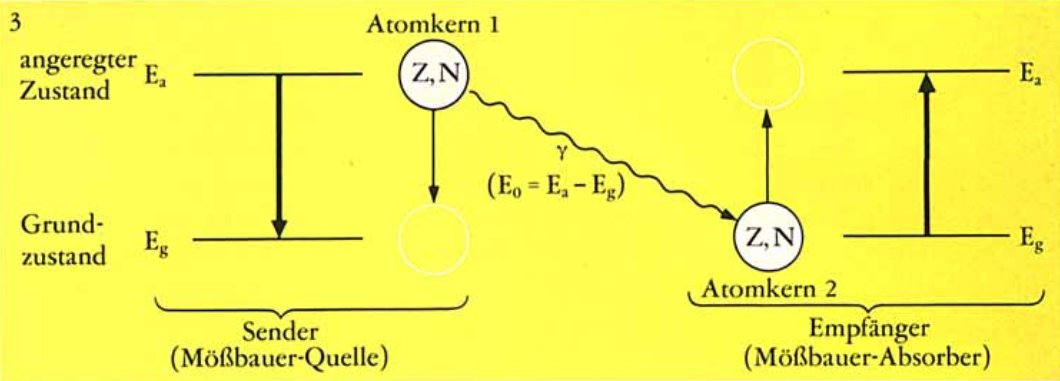
\includegraphics[scale=0.7]{Pic/Prinzip_Kernresonanzabsorption}
\caption{Prinzip der Kernresonanzabsorption$\backslash$-emission${^{\cite{1}}}$}
\label{Kern}
\end{figure}
In Abblidung (\ref{Kern}) beschreibt schematisch die Kernresonanzabsorption$\backslash$-emission. 
Der Atomkern 1 ist im angeregtem Zustand mit Protonenzahl $Z$ und Neutronenzahl $N$ hat einen Energieinhalt ${E}_{{a}}$. 
Nach einer bestimmten Zeit $\tau$ geht dieser wieder in den Grundzustand zurück und hat damit einen Energieinhalt von ${E}_{{g}}$. 
Durch diesen Gamma-Zerfall wird Energie $E_0 = {E}_{{a}}- {E}_{{g}}$ als Gamma-Quant freigesetzt. 
Dieser Gamma-Quant kann nun einen identischen Atomkern 2 vom Grundzustand in den angeregten Zustand überführen.
\newpage 
\begin{minipage}[t]{\textwidth}
\begin{wrapfigure}{l}{5cm}
\vspace{-20pt}
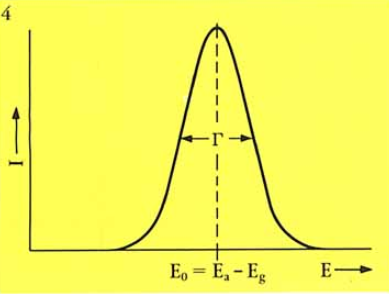
\includegraphics[scale=0.7]{Pic/Lorentz}
\caption{Intensität-Übergangsenergie-Diagramm für Kernübergänge${^{\cite{1}}}$}
\label{Lor}
\end{wrapfigure}
Für die Energieübergänge (und die dabei auftretenden Spektralinien) ist wichtig zu berücksichtigen,
dass diese den Gesetzen der Statistik unterliegen.
In Abbildung (\ref{Lor}) ist die Übergangswahrscheinlichkeit (bzw. die Intensität I) als Funktion der Übergangsenergie $E$ dargestellt.
Formell kann diese Funktion als:
\begin{align*}
I=\frac{const}{({E}-{E}_0)^2 + (\frac{\Gamma}{2})^2}
\end{align*}
Daher wird per Definition das Intensitätsmaximum  bei der Energiedifferenz 
${E}_0 = {E}_a - {E}_g$ gelegt, da dort die Übergangswahrscheinlichkeit (bzw. Intensität) am höchsten ist.
\end{minipage} 

Eine weitere charakteristische Größe ist hier das $\Gamma$, die sogenannte Halbwertsbreite. Diese ist ebenfalls in Abbildung (\ref{Lor}) zu sehen und entspricht der Linienbreite in halber Höhe des Intensitätsmaximum. 
Die Halbwertsbreite hat ein Minimum, welches durch die Heisenbergsche Unschärferela-\\ tion gegeben ist:
\begin{align*}
\Gamma_0\cdot\tau = \hbar{,}
\end{align*}
mit $\tau$ der Lebensdauer des ang. Zustandes. 
Die für den Mößbauereffekt beobachteten $\gamma$-Quanten bei Kernübergängen haben sowohl bei der Emission als auch bei der Absorption genau diese Lorentzform. Der Mößbauereffekt benötigt zusätzlich noch, dass die Emissions- und Absorptionslinie sich möglichst weitgehend überschneiden, da dort der Resonanzeffekt am größten ist. \par

Wichtig für den Mößbauereffekt ist, dass die Kernresonanzabsorption$\backslash$-emission rückstoßfrei ist. Dies ist aber oft nicht der Fall, da der angeregte Atomkern bei Emission eines $\gamma$-Quants einen Impuls $p$ und nach der Formel $E=\vert p \vert \cdot c$ eine Rückstoßenergie $\text{E}_{\text{R}}$ erfährt. Diese Rückstoßenergie vermindert nun die vom emittierten $\gamma$-Quant mitgenommene Energie ${E}_{\gamma} = {E}_0 - {E}_{{R}}$. Dies hat nun zur Folge, dass die Emissions- und Absorptionslinie nicht an der Stelle ${E}_0$ auftreten, sondern um $\vert {E}_{{R}} \vert$ verschoben. 
\newpage
\begin{minipage}[t]{\textwidth}
\begin{wrapfigure}{l}{8cm}
\vspace{-20pt}
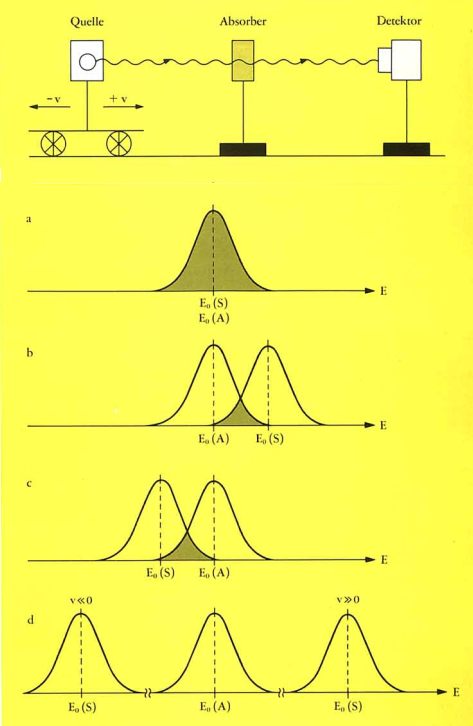
\includegraphics[scale=0.9]{Pic/Versuch}
\caption{Prinzip Mößbauereffekt${^{\cite{1}}}$}
\label{Mos}
\end{wrapfigure}
Um der Verschiebung entgegenzuwirken, kann man den Versuchsaufbau wie in Abbildung (\ref{Mos}) betrachten.
Anstatt Quell- und Absorberatomkerne statisch zu betrachten, kann man einfach eines der beiden, im Falle der Abbildung die Quelle, dynamisch verschieben. Da die Rückstoßenergie eine Tranlationsenergie ist, wird ${E}_{{R}}=0$ für eine Relativgeschwindigkeit $v=0$. An diesem Punkt (Abbildung (\ref{Mos}a)) überlappen sich die Emissions- und Absorptionsline maximal. Ist die Relativgeschwindigkeit im Betrag größer als Null, so tritt je nach Vorzeichen Fall b) oder c) auf und erweitert sich für $v>>0$ auf den Fall d).\par
\end{minipage} \\
~\\
\vspace{150pt}~\\
\begin{minipage}[t]{\textwidth}
\begin{wrapfigure}{r}{6cm}
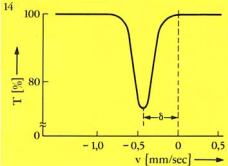
\includegraphics[scale=1.5]{Pic/Isomerie}
\caption{Mößbauerspektrum von $\text{K}_4[\text{Fe(CN)}_6]\cdot 3\text{H}_2\text{O}$~${^{\cite{1}}}$}
\label{Iso}
\end{wrapfigure}
Während der Kernübergänge wird praktisch niemals der nackte Atomkern getroffen und weiter ist der Atomkern nicht punktförmig, sondern hat eine räumliche Ausdehnung. Daher tritt bei Kernübergängen praktisch nie $\text{E}_0$ sondern ein gegenüber ${E}_0$ verschobene Energie ${E}_{{S}}$ für die Emission bzw. ${E}_{{A}}$ bei der Absorption auf. Die Ursache dafür ist die Monopolwechselwirkung zwischen Atomkernen und Elektronen am Kernort. Dies ergibt sich aus zwei Folgerungen. Zum einen bewegen sich Elektronen auch im Atomkern. Daher kann man auch eine Elektronendichte für den Kern definieren, in dem wir die Wellenfunktion $\Psi(r)$ im Quadrat an der Stelle $r=0$ betrachten. Weiter erfährt der angeregte Kern eine räumliche Ausdehnung ${R}_{{a}}$ die größer ist als die im Grundzustand ${R}_{{g}}$. Dies ergibt dann eine Enegiedifferenz $\Delta E(S)$ (bzw. aus Analogiegründen $\Delta E(A)$) welche wie folgt mathematische beschrieben werden kann.
\end{minipage}
\newpage
\begin{align*}
\Delta E(S)&=const\cdot \vert \Psi(0)\vert^2_{{S}}\cdot({R}_{{a}}^2-{R}_{{g}}^2) \\
\Delta E(A)&=const\cdot \vert \Psi(0)\vert^2_{{A}}\cdot({R}_{{a}}^2-{R}_{{g}}^2) 
\end{align*}
Die Isomerieverschiebung $\delta$ ist nun die Differenz
\begin{align*}
\delta = \Delta E(A)- \Delta E(S) = const\cdot (\vert \Psi(0)\vert^2_{{A}}-\Psi(0)\vert^2_{{S}})\cdot({R}_{{a}}^2-{R}_{{g}}^2) = {E}_{{A}}-{E}_{{S}}
\end{align*}
und ist ein Maß für die Veränderung der Valenzschale, also Änderungen im Oxidationszustand oder in den Bindungsverhältnissen und kann mit Hilfe des Mößbauereffekts gemessen werden.

Mit dem Mößbauereffekt ist ebenso eine Quadrupolaufspaltung bei bestimmten Atomen zu beobachten. Legt man ein inhomogenes elektrisches Feld am Kernort an, so wechselwirkt dies mit dem Quadropolmoment $Q$ des Kerns. Daraufhin spalten sich die Kernenergieniveaus in ($I$+1/2), $I$ Kernspin, Subniveaus auf. Für die Chemie und Festkörperphysik ist der elektrische Feldgradient, welcher ein Maß für die Inhomogenität des elektrischen Feldes am Kernort ist, eine wichtige Anwendung der Mößbauerspektroskopie, da man dadurch Rückschlüsse unter andere auf die Molekülsymmetrie ziehen kann. Nimmt man an, dass die Inhomogenität des elektrischen Feldes sich als axialsymmetrisches Feldgefälle behandeln lässt, so gilt für die einzelnen Niveaus:
\begin{align*}
E_Q = \frac{eqQ}{4I(2I-1)}[3m_l^2-I(I+1)]
\end{align*}
und für den elektrischen Feldgradienten $q$ ist es oft einfacher, die Energiedifferenz $\Delta E_Q$ sich anzuschauen.

Eine weitere Information, welche mit Hilfe des Mößbauereffekts sich in Erfahrung bringen lassen kann, ist das magnetische Verhalten und daraus z.B. die Wertigkeit. Dies tritt durch magnetische Wechselwirkung zwischen dem magnetischen Dipolmoment $\mu$ des Kerns und einem magnetischen Feld der Stärke $H$ am Kernort auf. Die Kernenergieniveaus werden dann in $(2I+1)$ Subniveaus, sogenannten Hyperfeinniveaus, aufgespalten, wobei die einzelnen Niveaus durch ihre magnetische Spinquantenzahl $m_I$ charakterisiert sind.
Die einzelnen Hyperfeinenergieniveaus sind durch die Formel 
\begin{align*}
E_M = -\mu H \frac{m_I}{I}
\end{align*}
gegeben und die Gesamtaufspaltung $\Delta E_M$ (Abstand
zwischen den beiden äußersten Linien) ist daher proportional zur Magnetfeldstärke.


\newpage

\begin{minipage}{0.5\textwidth}
\begin{figure}[H]
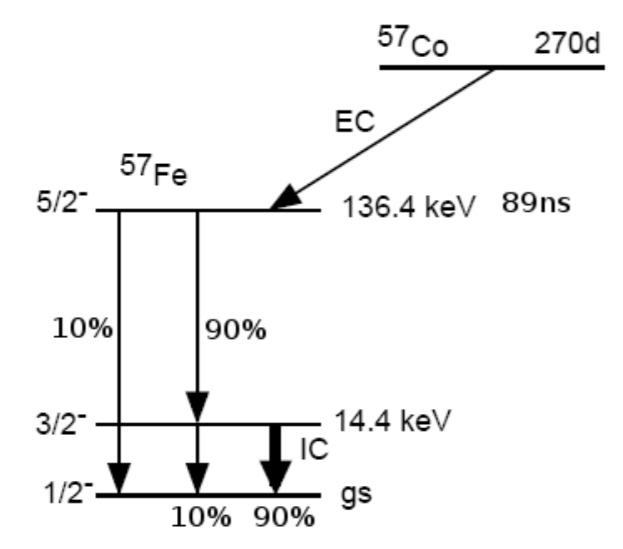
\includegraphics[scale=0.5]{Pic/Termschema} 
\label{Term}
\caption{Das Zerfallsschema von $^{57}$Co$^{\cite{4}}$}
\end{figure}
\end{minipage}
\begin{minipage}{0.5\textwidth}
In Abblidung (5) ist nun das Zerfallsschema von $^{57}$Co zu sehen. Der Übergang von $I=\frac{5}{2}$ nach $I=\frac{1}{2}$ ist ein Gamma-Zerfall mit einer Energie von 136.4~,keV, der Aufgrund von Statistik auftritt, obwohl er nach den Übergangsregeln verboten ist. Weiter gibt es den Übergang von $I=\frac{5}{2}$ nach $I=\frac{3}{2}$. Diese sind ebenso Gammazerfälle bei 122\,keV und 14.4\,keV. Der Übergang von $I=\frac{3}{2}$ nach $I=\frac{1}{2}$ ist die innere Konversion, eine besondere Art der Radioaktivität, die in unserem Versuch nicht detektierbar ist.
\end{minipage}


\section{Versuchsaufbau \& Versuchsbeschreibung}

\begin{figure}[H]
\centering
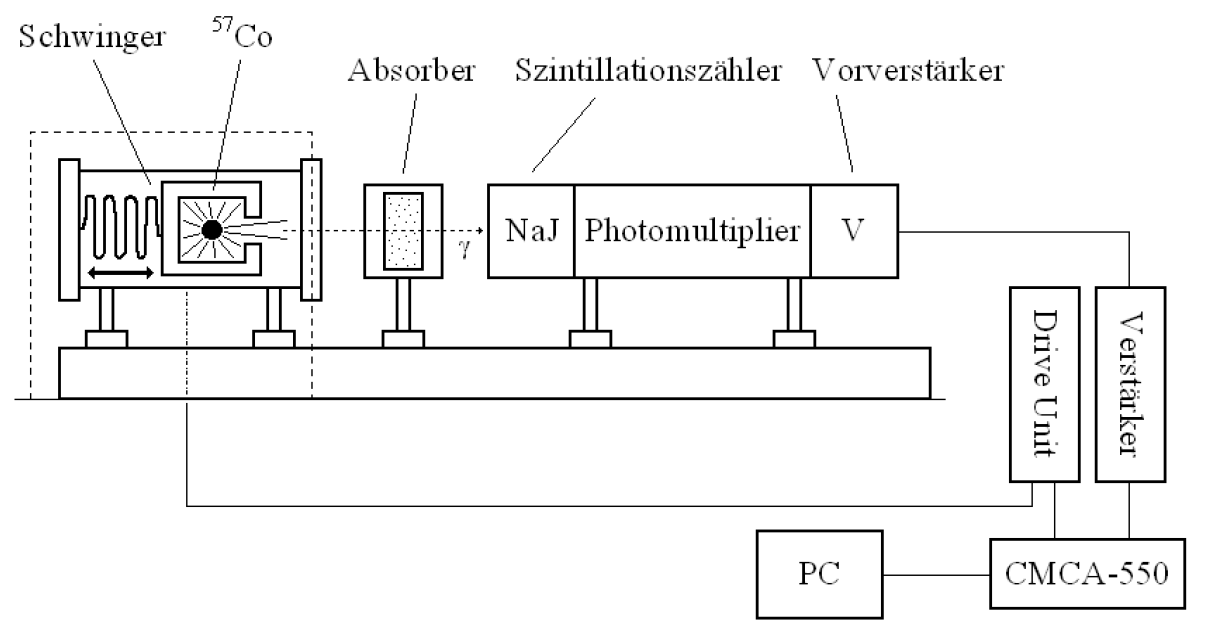
\includegraphics[scale=0.4]{Pic/Aufbau}
\caption{Schematischer Versuchsaufbau${^{\cite{3}}}$}
\label{Aufbau}
\end{figure}
In Abbildung (\ref{Aufbau}) ist der Aufbau des Versuchs zu sehen. Das $^{57}$Co ist an einer schwingenden Achse eines elektromagnetischen Schwingers befestigt, welcher mit einer einstellbaren Frequenz schwingen kann. Der Schwinger ist mit dem Vielkanalanalysator (CMCA-550) synchronisiert, sodass jeder einzelne Kanal einer bestimmten Momentangeschwindigkeit der Quelle zugeordnet ist. 

Im ersten Teil des Versuchs wird kein Absorber verwendet, was uns die Messung des Gamma-Spektrums von $^{57}$Co ermöglicht. Im zweiten Teil werden verschiedene Absorber verwendet um die verschiedenen Effekte des Mößbauereffekts zu sehen.

\newpage

\section{Auswertung}

\subsection{Gamma-Spektrum von $^{57}$Co}

\begin{figure}[H]
\centering
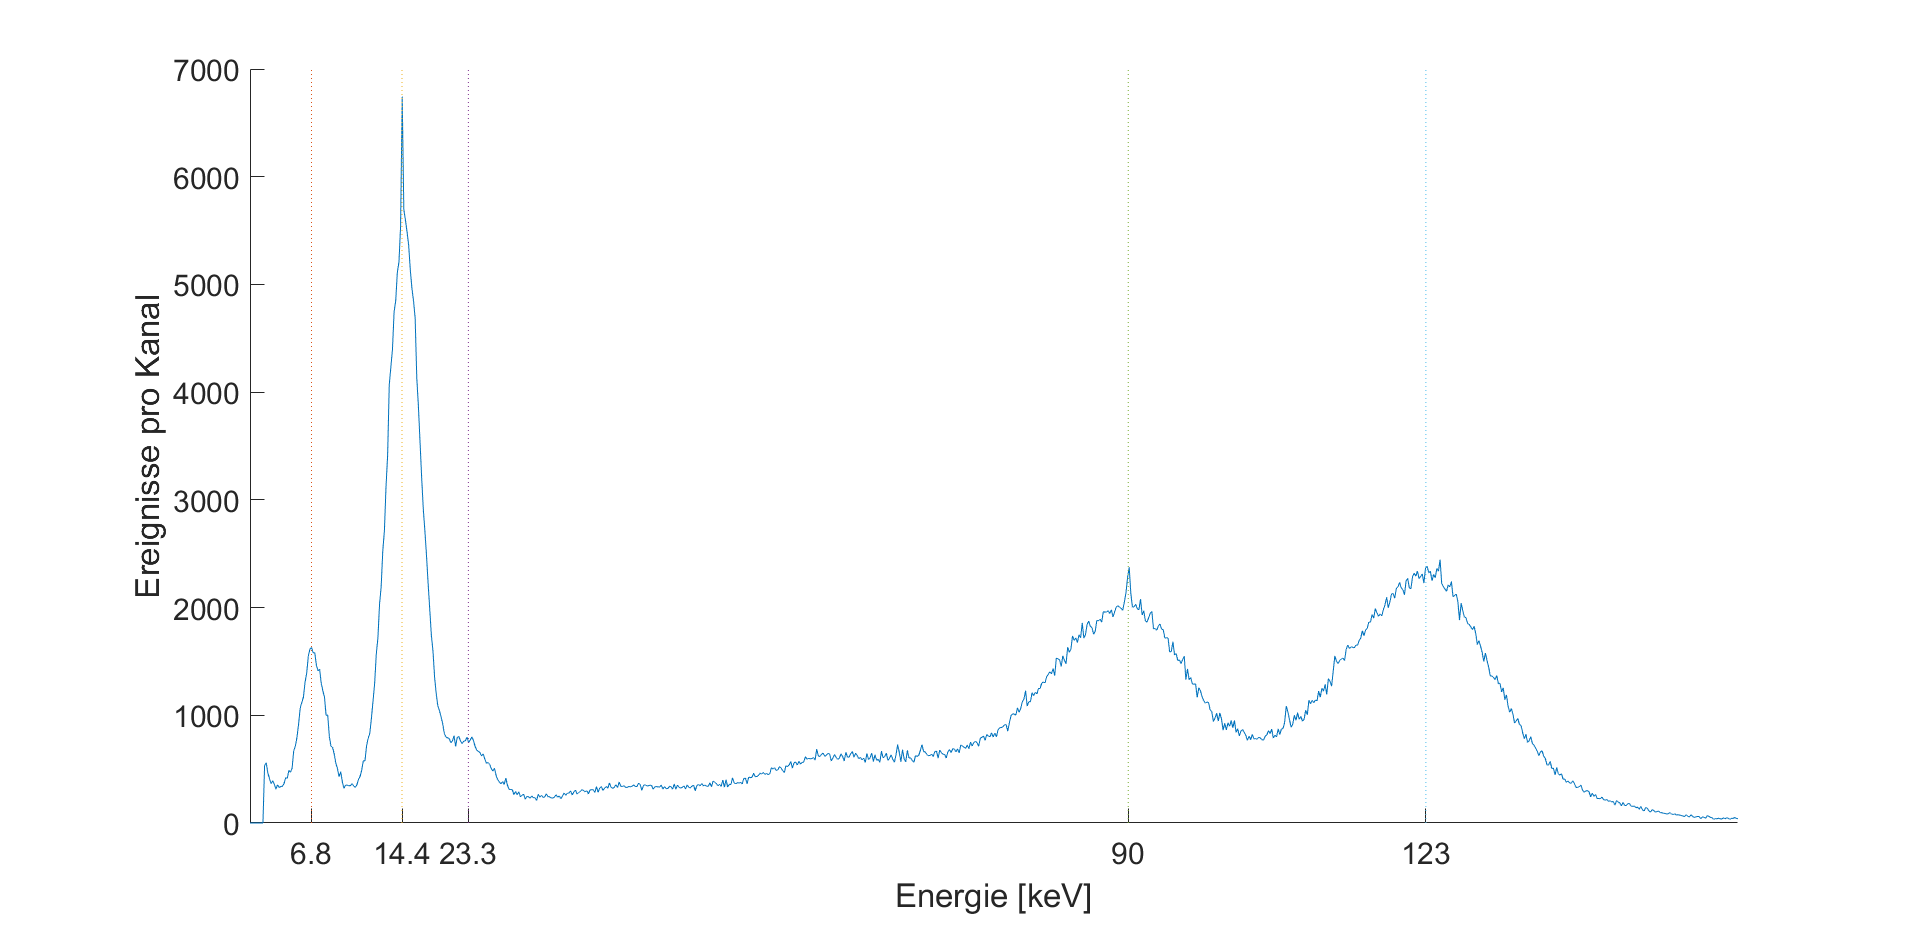
\includegraphics[scale=0.3]{Pic/Gamma}
\caption{Messergebnisse: Gamma-Spektrum von $^{57}$Co}
\label{Gamma}
\end{figure}

In ersten Versuchsteil wurde das Gammaspektrum von $^{57}$Co gemessen, welches in Abbildung (\ref{Gamma}) dargestellt wird. Es sind 5 Peaks beobachtbar. Der erste tritt bei etwa 6.8\,keV auf und ist technisch bedingt, da in diesem Versuch das $^{57}$Co durch K-Einfang in den angeregten Zustand von $^{57}$Fe übergeht. Das angeregte $^{57}$Fe ($I$=3/2) setzt Gamma-Quanten frei um in den Grundzustand ($I$=1/2) zu gelangen, welche den zweite Peak bei etwa 14.4\,keV erklären. Ein dritter Peak ist bei etwa 23.3\,keV zu betrachten und begründet sich dadurch, dass unser $^{57}$Co in Rhodium eingebttet ist, welches ebenfalls strahlt. Ein weiterer Peak, der bei uns bei genau 90\,keV liegt, ist wieder technisch bedingt und dem Szintillationszähler geschuldet. Der letzte Peak bei etwa 123\,keV ensteht durch Emission von $I$=5/2 nach 
$I$=3/2.

\newpage

\subsection{Hyperfeinstrukturaufspaltung von $^{57}$Fe}

\begin{figure}[H]
\centering
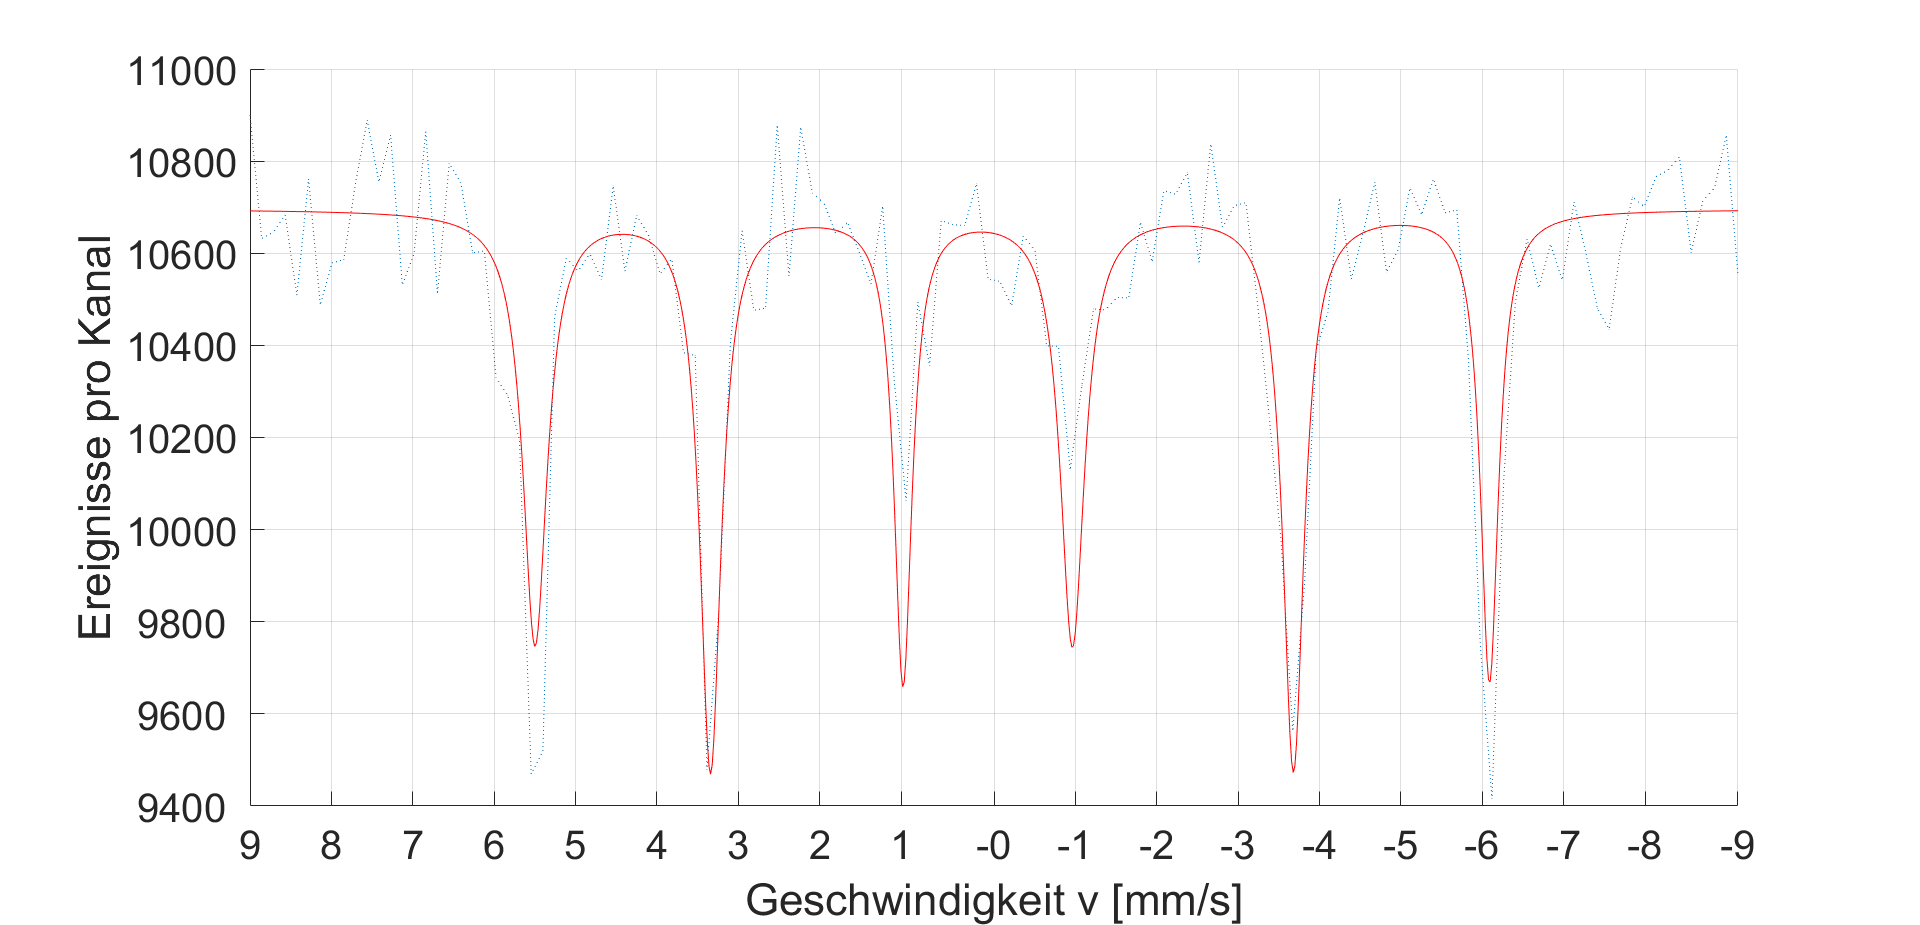
\includegraphics[scale=0.3]{Pic/Hyper}
\caption{Messergebnisse: Hyperfeinstrukturaufspaltung von $^{57}$Fe}
\label{Hyper}
\end{figure}

In Abblidung (\ref{Hyper}) ist unsere Messung zur Hyperfeinstrukturaufspaltung von $^{57}$Fe zu betrachten. Zuallererst berechnen wir die Isomerieverschiebung. Dazu wurde ein Lorentzfit mit 6 Peaks genommen. Diese Peaks erlauben uns dann, durch Differenzbetrachtung, die Isomerieverschiebung $\delta=\frac{\vert v_{\text{rechts}} \vert - \vert v_{\text{links}} \vert }{2}$ zu bestimmen. In folgender Tabelle werden alle wichtigen Werte benannt, wobei hier schon die Peaks geordnet wurden:

\begin{figure}[H]
\centering
\begin{tabular}{c|c||c}
\hline 
\rule[-1ex]{0pt}{2.5ex} linke Seite $v$\,[$\frac{\text{mm}}{\text{s}}$] & rechte Seite $v$\,[$\frac{\text{mm}}{\text{s}}$] & Isomerieverschiebung $\delta$\,[$\frac{\text{mm}}{\text{s}}$]  \\ 
\hline 
\rule[-1ex]{0pt}{2.5ex} 5,55 & -5,99 & -0,220 \\ 
\hline 
\rule[-1ex]{0pt}{2.5ex} 3,43 & -3,62 & -0,095 \\ 
\hline 
\rule[-1ex]{0pt}{2.5ex} 0,95 & -1,10 & -0,075 \\ 
\hline 
\hline 
\multicolumn{2}{c||}{\textbf{Mittelwert:}} & -0,13 \\ 
\hline 
\end{tabular} 
\caption{Messwerte: Lorentzpeaks}
\end{figure}
Weiter ist zu beachten, dass wir einen kleinen berechenbaren Fehler in unseren Messungen haben. Da wir 128 Kanäle haben und wir von -9\,$\frac{\text{mm}}{\text{s}}$ bis 9\,$\frac{\text{mm}}{\text{s}}$ gehen, ist der Fehler
\begin{align*}
\Delta v = \frac{18\,\frac{\text{mm}}{\text{s}}}{128} \approx0,14\,\frac{\text{mm}}{\text{s}}.
\end{align*}
Somit ist unsere Abblidung (\ref{Hyper}) um $v=(-0,13\pm0,14)\,\frac{\text{mm}}{\text{s}}$ symmetrisch. Dies ergibt dann dann für die Energie $\text{E}_{\text{D}}$, um welche
die Energie $\text{E}_{\text{S}}$
der emittierten Gamma-Quanten durch Bewegung
der Quelle relativ zum Absorber verändert
werden muss um
\begin{align*}
{E}_{{D}} = E_S\cdot\frac{v}{c} = 14,4\,\text{keV}\cdot\frac{(-0,13\pm0,14)\,\frac{\text{mm}}{\text{s}}}{3\cdot 10^{11} \frac{\text{mm}}{\text{s}} } = (-6,24\pm 6,72)\cdot 10^{-9}\,\text{eV}{.}
\end{align*} 

Weiter können wir nach der Formel 
\begin{align*}
\Delta E_M = - H \Delta \left( \frac{m_I}{I}\mu \right) \quad \imp \quad \frac{v}{c} = E_M + \frac{H}{{E}_{{S}}} \left( \frac{\mu_g m_g}{I_g}-\frac{\mu_e m_e}{I_e} \right){,}
\end{align*}
unter Beirücksichtung der Tatsache, dass wir einen Zerfall von $I$=3/2 nach $I$=1/2 und den Auswahlregeln $\Delta m = \pm 1$ durch Umformung auf folgende Formel zurückschließen:
\begin{align*}
v_4 - v_2 = v_5 - v_3 = \frac{2\mu_g H c}{\text{E}_{\text{S}}}{.}
\end{align*}
Darum ist das Magnetfeld am Kernort durch die Formel 
\begin{align*}
H = \frac{{E}_{{S}} (v_4 - v_2) }{2c\mu_g}
\end{align*}
gegeben, wobei $\mu_g=0,0903\mu_k$ laut Versuchsanleitung ist. Mit unserem Fehler von $\Delta v =0,14\,\frac{\text{mm}}{\text{s}}$ ergibt sich damit:
\begin{align*}
H =\frac{14,4\cdot 10^3\,\text{eV}\cdot (0,95-(-3,62))\frac{\text{mm}}{\text{s}} }{2\cdot 3\cdot 10^{11}\frac{\text{mm}}{\text{s}}\cdot 0,0903\cdot 3,52\cdot 10^{-8}\frac{\text{eV}}{\text{T}} } = (34,58\pm 2,114)\,\text{T}
\end{align*}

Zu guter Letzt berechnen wir nun das fehlende $\mu_e$, dass wir wieder durch Umformen der Gleichung für $\Delta E_M$ erhalten. Es gilt allgemein:
\begin{align*}
\mu_{e_1} &= 3 \frac{v_2-v_{1}}{v_4-v_2}\cdot\mu_g = -0,13\mu_k \\
\mu_{e_2} &= 3 \frac{v_3-v_{2}}{v_4-v_2}\cdot\mu_g = -0,14\mu_k \\
\mu_{e_3} &= 3 \frac{v_5-v_{4}}{v_4-v_2}\cdot\mu_g = -0,17\mu_k \\
\mu_{e_4} &= 3 \frac{v_6-v_{5}}{v_4-v_2}\cdot\mu_g = -0,15\mu_k \\
\mu_{e_5} &= \frac{3}{2} \frac{v_3-v_{1}}{v_4-v_2}\cdot\mu_g = -0,14\mu_k \\
\mu_{e_6} &= \frac{3}{2} \frac{v_6-v_{4}}{v_4-v_2}\cdot\mu_g = -0,16\mu_k \\
\end{align*}
Wodurch sich als Mittelwert nun der Wert $\mu_e = -0,1483\mu_k$ ergibt.

\subsection{Geschwindigkeitskalibrierung}

Die Geschwindigkeitsmessungen in diesem Versuch sind nicht ganz genau, daher müssen wir vorher eine Geschwindigkeitskalibrierung vornehmen. Diese lässt sich berechnen durch
\begin{align*}
f_{\text{kal.}} =\frac{\Delta v_{lit}}{v_6-v_1}=\frac{10,6\,\frac{\text{mm}}{\text{s}}}{(5,55-(-5,99))}\frac{\text{mm}}{\text{s}} = 0,92.
\end{align*}


\subsection{Isomerieverschiebung und elektrischer Feldgradient bei FeSO$_4\cdot$7H$_2$O}

\begin{figure}[H]
\centering
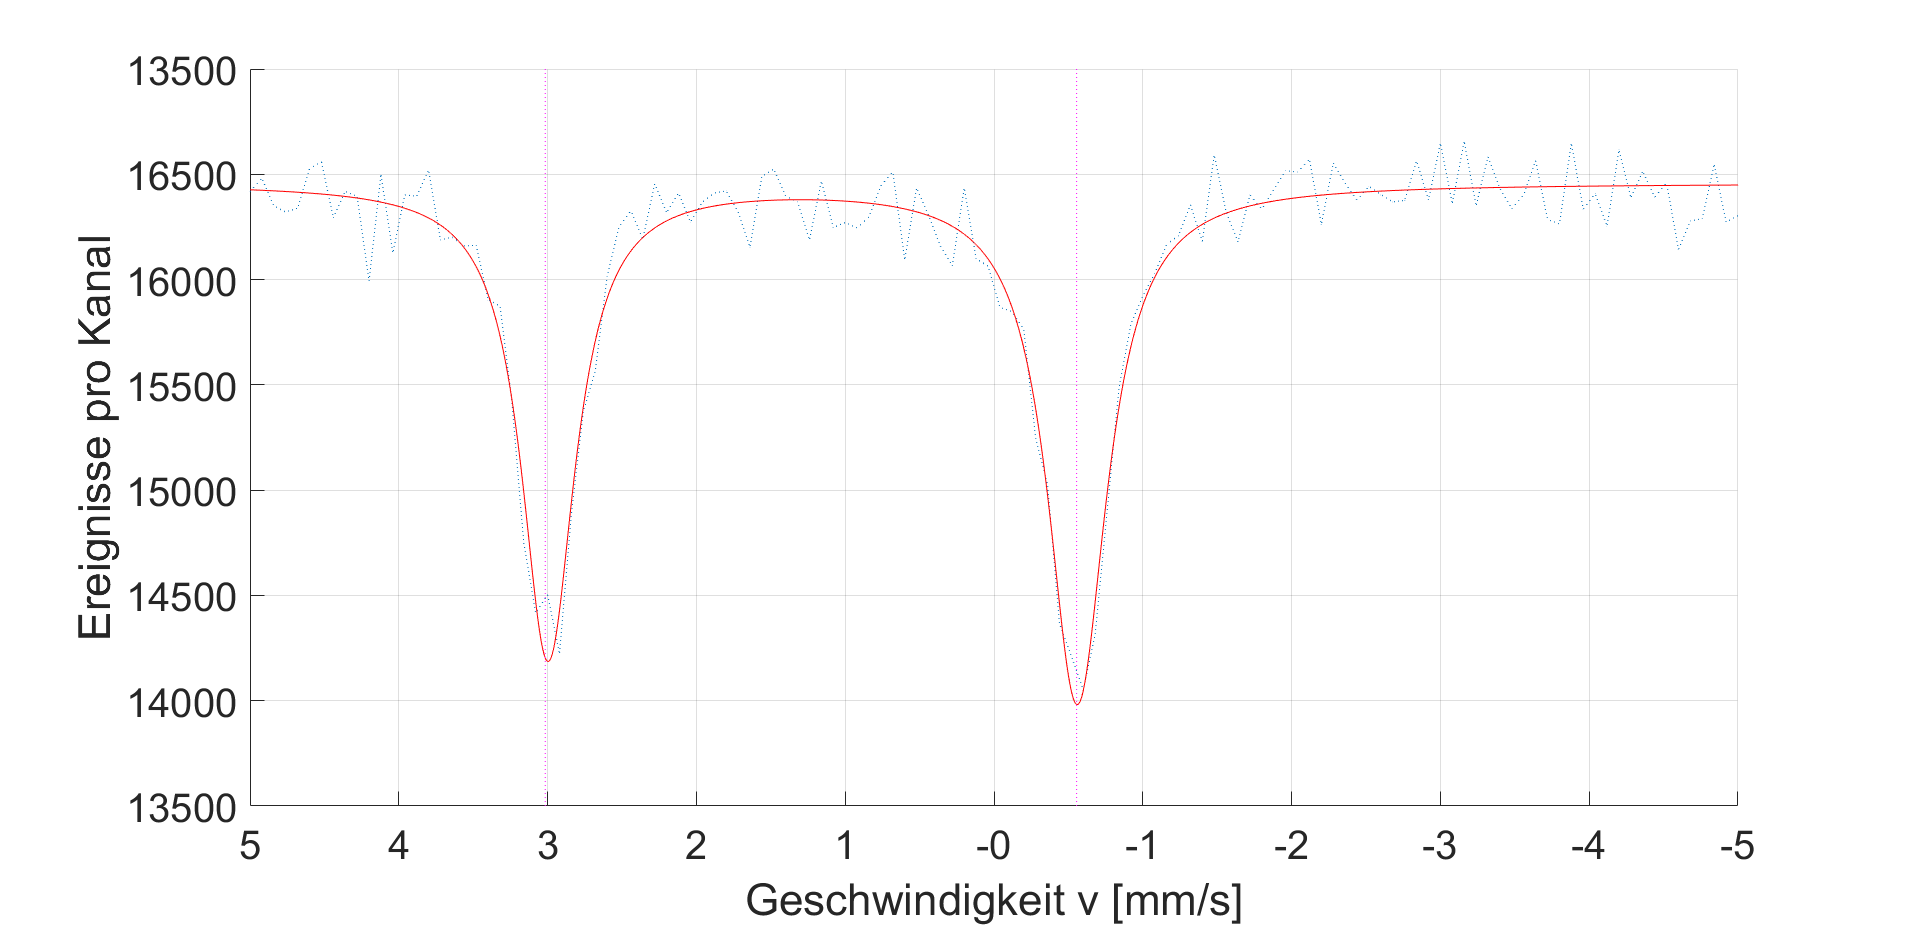
\includegraphics[scale=0.3]{Pic/Feso}
\caption{Messergebnisse: Spektrum von FeSO$_4\cdot$7H$_2$O}
\label{Feso}
\end{figure}

Das gemessene Spektrum ist in Abblidung (\ref{Feso}) abgebildet. Zuallererst berechnen wir die Isomerieverschiebung. Dafür gehen wir genauso vor wie bei dem natürlichen Eisen. Aus den Lorentzfits ergibt sich:
\begin{figure}[H]
\centering
\begin{tabular}{c|c||c}
\hline 
\rule[-1ex]{0pt}{2.5ex} linke Seite $v$\,[$\frac{\text{mm}}{\text{s}}$] & rechte Seite $v$\,[$\frac{\text{mm}}{\text{s}}$] & Isomerieverschiebung $\delta$\,[$\frac{\text{mm}}{\text{s}}$]  \\ 
\hline 
\rule[-1ex]{0pt}{2.5ex} 2,9968 & -0,5595 & 1,22 \\ 
\hline 
\end{tabular} 
\caption{Messwerte: Lorentzpeaks}
\end{figure}
Weiter ergibt sich ein Fehler von:
\begin{align*}
\Delta v = \frac{10\,\frac{\text{mm}}{\text{s}}}{128} = 0,0781\,\frac{\text{mm}}{\text{s}}.
\end{align*}
Wodurch $v=(1,22\pm 0,0781)\,\frac{\text{mm}}{\text{s}}$
beträgt und damit ergibt sich für ${E}_{{D}}$:
\begin{align*}
{E}_{{D}} = E_S\cdot\frac{v}{c} = 14,4\,\text{keV}\cdot\frac{(1,22\pm0,0781)\,\frac{\text{mm}}{\text{s}}}{3\cdot 10^{11} \frac{\text{mm}}{\text{s}} } = (58,56\pm 3,75)\cdot 10^{-9}\,\text{eV}.
\end{align*} 

Um nun den elektrischen Feldgradienten zu bestimmen, verwenden wir die Formel wie in der Theorie genannt und schauen uns die Differenz an. Es gilt:
\begin{align*}
{E}_{{Q}} = E_Q(I=3/2; m_I=\pm 3/2)- E_Q(I=3/2; m_I=\pm 1/2) = \frac{eqQ}{2} = {E}_{{S}}\frac{v_2-v_1}{c}.
\end{align*}
Durch Umformen dieser Gleichung kann der elektrische Feldgradient berechnet werden:
\begin{align*}
q&=\frac{2{E}_{{S}}\frac{(v_2-v_1)+\Delta v}{c}}{eQ} = \frac{2 \cdot \vert (-0,5595-(+2,9968)\vert \pm 0,0781)\,\frac{\text{mm}}{\text{s}}\cdot 14,4\cdot10^3\,\text{eV}}{1\,\frac{\text{eV}}{V}\cdot 0,29\cdot 10 ^{-28}\,\text{m}^2\cdot  3\cdot 10^{11}\frac{\text{mm}}{\text{s}} } \\ &= (1,1773\pm 0,0517) \cdot 10^{22}\,\frac{\text{V}}{\text{m}^2}.
\end{align*}
Hierbei wurde wieder als Fehler $\Delta v =0,0781\,\frac{\text{mm}}{\text{s}}$ genommen und ein Wert aus der Versuchsanleitung, nämlich $Q=0,29\cdot 10 ^{-28}\,\text{m}^2$, genommen.

\subsection{Isomerieverschiebung von K$_4$(Fe(CN)$_6$)$\cdot$3H$_2$O }

\begin{figure}[H]
\centering
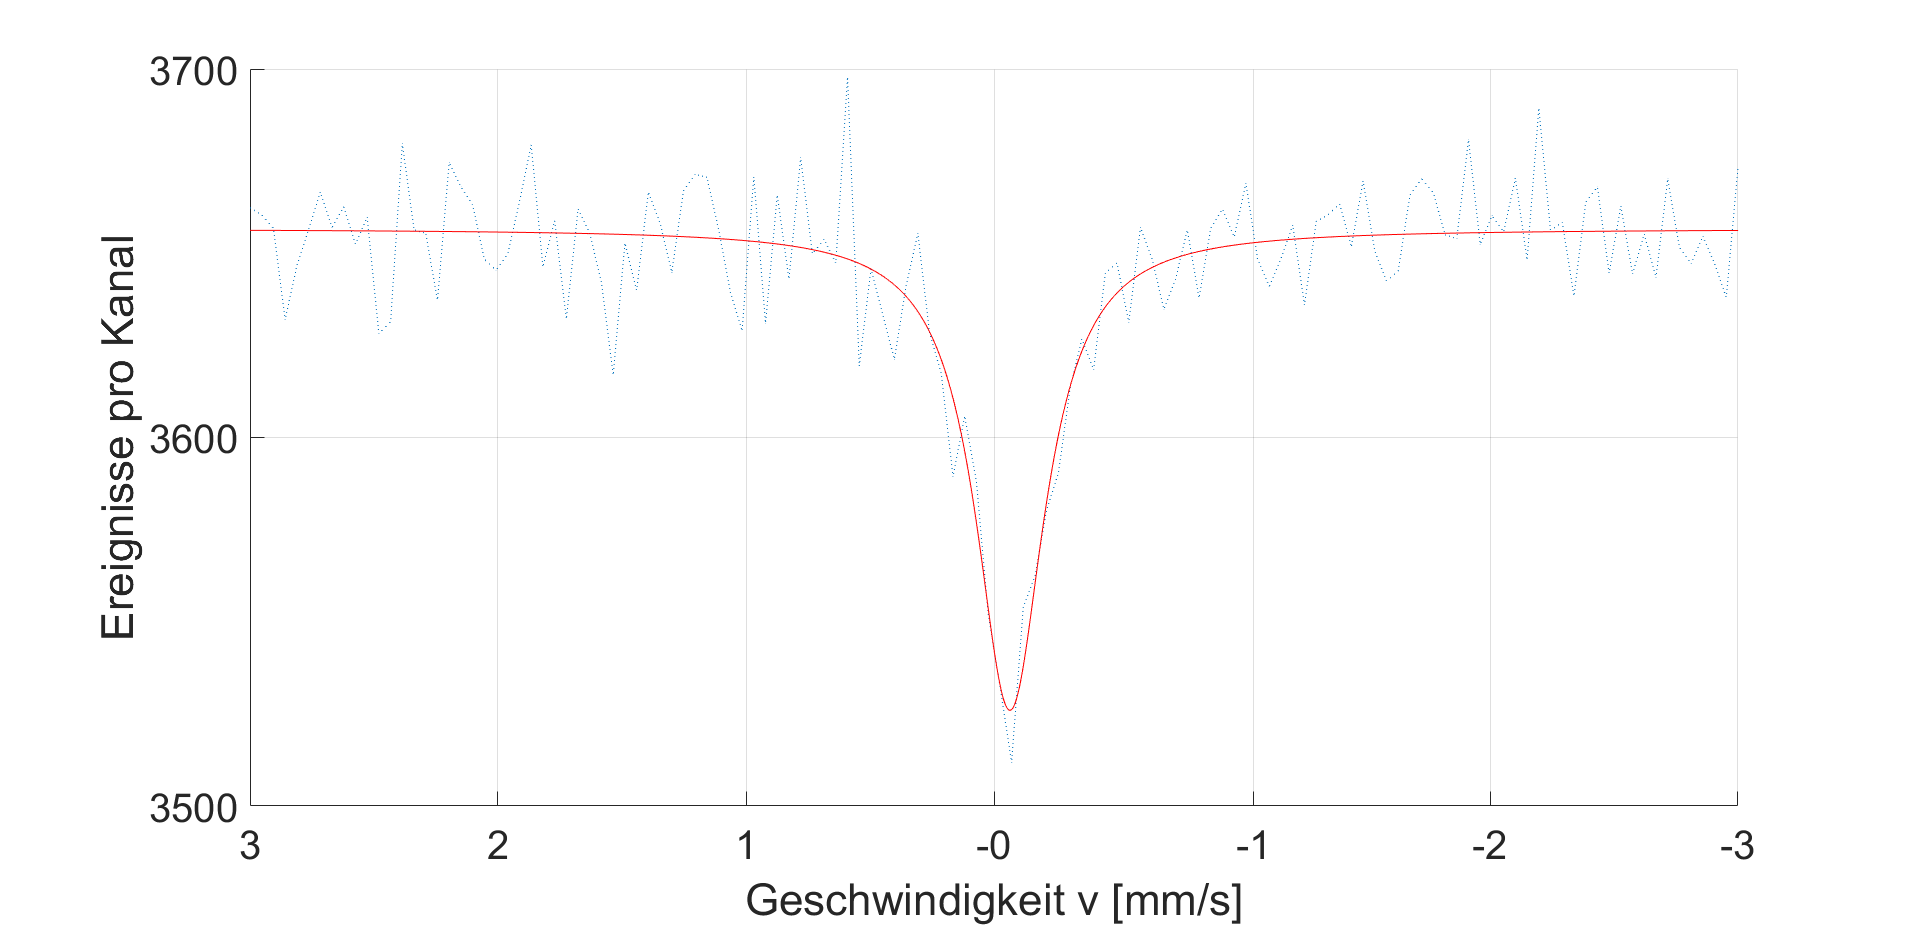
\includegraphics[scale=0.3]{Pic/K4}
\caption{Messergebnisse: Spektrum von K$_4$(Fe(CN)$_6$)$\cdot$3H$_2$O}
\label{K4}
\end{figure}

Laut Lorentzfit ist die Isomerieverschiebung $\delta=-0,0642\,\frac{\text{mm}}{\text{s}}$ mit dem Fehler $\Delta v= \frac{6\,\frac{\text{mm}}{\text{s}}}{128}=0,0469\,\frac{\text{mm}}{\text{s}}$.



\section{Fehlerbetrachtung}

Alle nötigen Fehlerfortpflanzungen wurden schon im Auswertungsteil mit berechnet. Ansonsten ist der Versuch recht abgeriegelt, so dass keine Fehler bei der Durchführung möglich sind.

\section{Zusammenfassung}

Im ersten Teil des Versuchs haben wir uns das Gamma-Spektrum von $^{57}$Co angeschaut und erklärt. Danach haben wir das natürliche Eisen $^{57}$Fe angeschaut. Wir bekamen eine Isomerieverschiebung von
\begin{align*}
v=(-0,13\pm0,14)\,\frac{\text{mm}}{\text{s}}.
\end{align*}
Laut Literatur ist liegt dieser bei
\begin{align*}
\delta(\text{Rh},\text{Fe})=-0,11\,\frac{\text{mm}}{\text{s}},
\end{align*}
womit wir eine relativ kleine Abweichung haben. Für das Magnetfeld am Kernort haben wir
\begin{align*}
H=(34,58\pm 2,114)\,\text{T}
\end{align*}
herausbekommen und der magnetische Moment des angeregten natürlichen Eisens war
\begin{align*}
\mu_e = -0,1483\mu_k.
\end{align*}

Im nächsten Abschnitt haben wir uns mit FeSO$_4\cdot$7H$_2$O beschäftigt. Für die Isomerieverschiebung ergab sich bei uns:
\begin{align*}
v=(1,22\pm 0,0781)\,\frac{\text{mm}}{\text{s}}.
\end{align*}
Nach Literatur ist dieser
\begin{align*}
\delta(\text{Fe},\text{FeSO}_4\cdot7\text{H}_2\text{O})&= \delta(\text{Rh},\text{Fe}) + \delta(\text{Fe},\text{Pt}) +\delta(\text{Pt},\text{FeSO}_4\cdot7\text{H}_2\text{O}) \\ &= (-0,11+0,35+0,92)\,\frac{\text{mm}}{\text{s}} \\ &= 1,16\,\frac{\text{mm}}{\text{s}}.
\end{align*}
Für die Quadrupolaufspaltung ergab sich bei uns:
\begin{align*}
\epsilon(\text{FeSO}_4\cdot7\text{H}_2\text{O})=0,5595\,\frac{\text{mm}}{\text{s}}+2,9968\,\frac{\text{mm}}{\text{s}}=3,5563\,\frac{\text{mm}}{\text{s}},
\end{align*}
wobei laut Literatur gilt:
\begin{align*}
\epsilon(\text{FeSO}_4\cdot7\text{H}_2\text{O})=3,19\,\frac{\text{mm}}{\text{s}}.
\end{align*}
Weiter haben wir für den elektrischen Feldgradienten 
\begin{align*}
q=(1,1773\pm 0,0517) \cdot 10^{22}\,\frac{\text{V}}{\text{m}^2}
\end{align*}
errechnet.\par 
Schlussendlich haben wir noch die Isomerieverschiebung von K$_4$(Fe(CN)$_6$)$\cdot$3H$_2$O betrachtet, welche bei uns bei 
\begin{align*}
v= -0,0642\pm0,0469\,\frac{\text{mm}}{\text{s}} 
\end{align*}
liegt. Laut Literatur gilt hier
\begin{align*}
\delta(\text{Fe},\text{K}_4\text{(Fe(CN)}_6)\cdot3\text{H}_2\text{O})&= \delta(\text{Fe},\text{Rh}) + \delta(\text{Fe},\text{Pt}) +\delta(\text{Pt},\text{K}_4\text{(Fe(CN)}_6)\cdot 3\text{H}_2\text{O}) \\ &= (-0,11+0,35-0,39)\,\frac{\text{mm}}{\text{s}} \\ &= -0,15\,\frac{\text{mm}}{\text{s}}.
\end{align*}


\renewcommand{\refname}{\textbf{Literaturverzeichnis}}
\begin{thebibliography}{xx}

 		  \bibitem[1]{1}		
\glqq Physikalische Methoden in der Chemie :
Mößbauer-Spektroskopie I\grqq ,\\
Chemie in unserer Zeit, Philipp Gütlich 
 	23.Juli.2018
 	
 	
    	 \bibitem[2]{2}			
\glqq Literaturwerte Isomerieverschiebung und Quadrupolaufspaltung\grqq ,
Universität Stuttgart (Hrsg.) Physikalisches Praktikum II: Versuchsanleitung. Universität Stuttgart.
2013.

 \bibitem[3]{3}			
\glqq schematischer Versuchsaufbau\grqq ,
Universität Stuttgart (Hrsg.) Physikalisches Praktikum II: Versuchsanleitung. Universität Stuttgart.
2013.

 \bibitem[4]{4}			
\glqq Termschema $^{57}$Co\grqq , \\
\emph{https://www.twam.info/wp-content/uploads/2009/04/fpraktikum-mos.pdf}.
2013.

\end{thebibliography}

\end{document}